% article example for classicthesis.sty
\documentclass[10pt,a4paper]{article} % KOMA-Script article scrartcl
\usepackage{lipsum}
\usepackage{url}
\usepackage[nochapters]{../classicthesis} % nochapters
\usepackage{graphicx}
\graphicspath{ {img/} }
\usepackage{booktabs}
\usepackage{float}
\usepackage{subfloat}
\usepackage{subfig}
\usepackage{hyperref}
\usepackage[ngerman]{babel}



\begin{document}
    \pagestyle{plain}
    \title{\rmfamily\normalfont\spacedallcaps{Mission: Chuckhole}}
    \author{\spacedlowsmallcaps{Marwan ElMezni, Michael Moosbauer}}
    \date{} % no date
    
    \maketitle
    
% picture titles still german

    \tableofcontents
    


    \section{Motivation and problem statement}

	

Even though municipalities try to maintain and repair roads, many segments still contain chuckholes that vehicle owners prefer to avoid to drive or to bike on because they would so likely damage their vehicles and slow or interrupt the traffic.\\
This was the background motivation to develop a mobile application, in a biking context, that helps users to avoid damaged sections of roads or to detect and localize chuckholes.

    \section{Recommended Setup}

	In order to use the main app \textbf{Mission:Chuckhole}, some requirements are needed.\\
	Of course, you need a bike to drive along the streets.
	For the test rides, two bikes have been used:

	\begin{itemize}
		\item \textbf{Dr"ossiger XRA 650 B}: full suspension All-Mountain-bike (150mm/155mm suspension)

		\begin{figure}[H]
		\begin{center}
 		  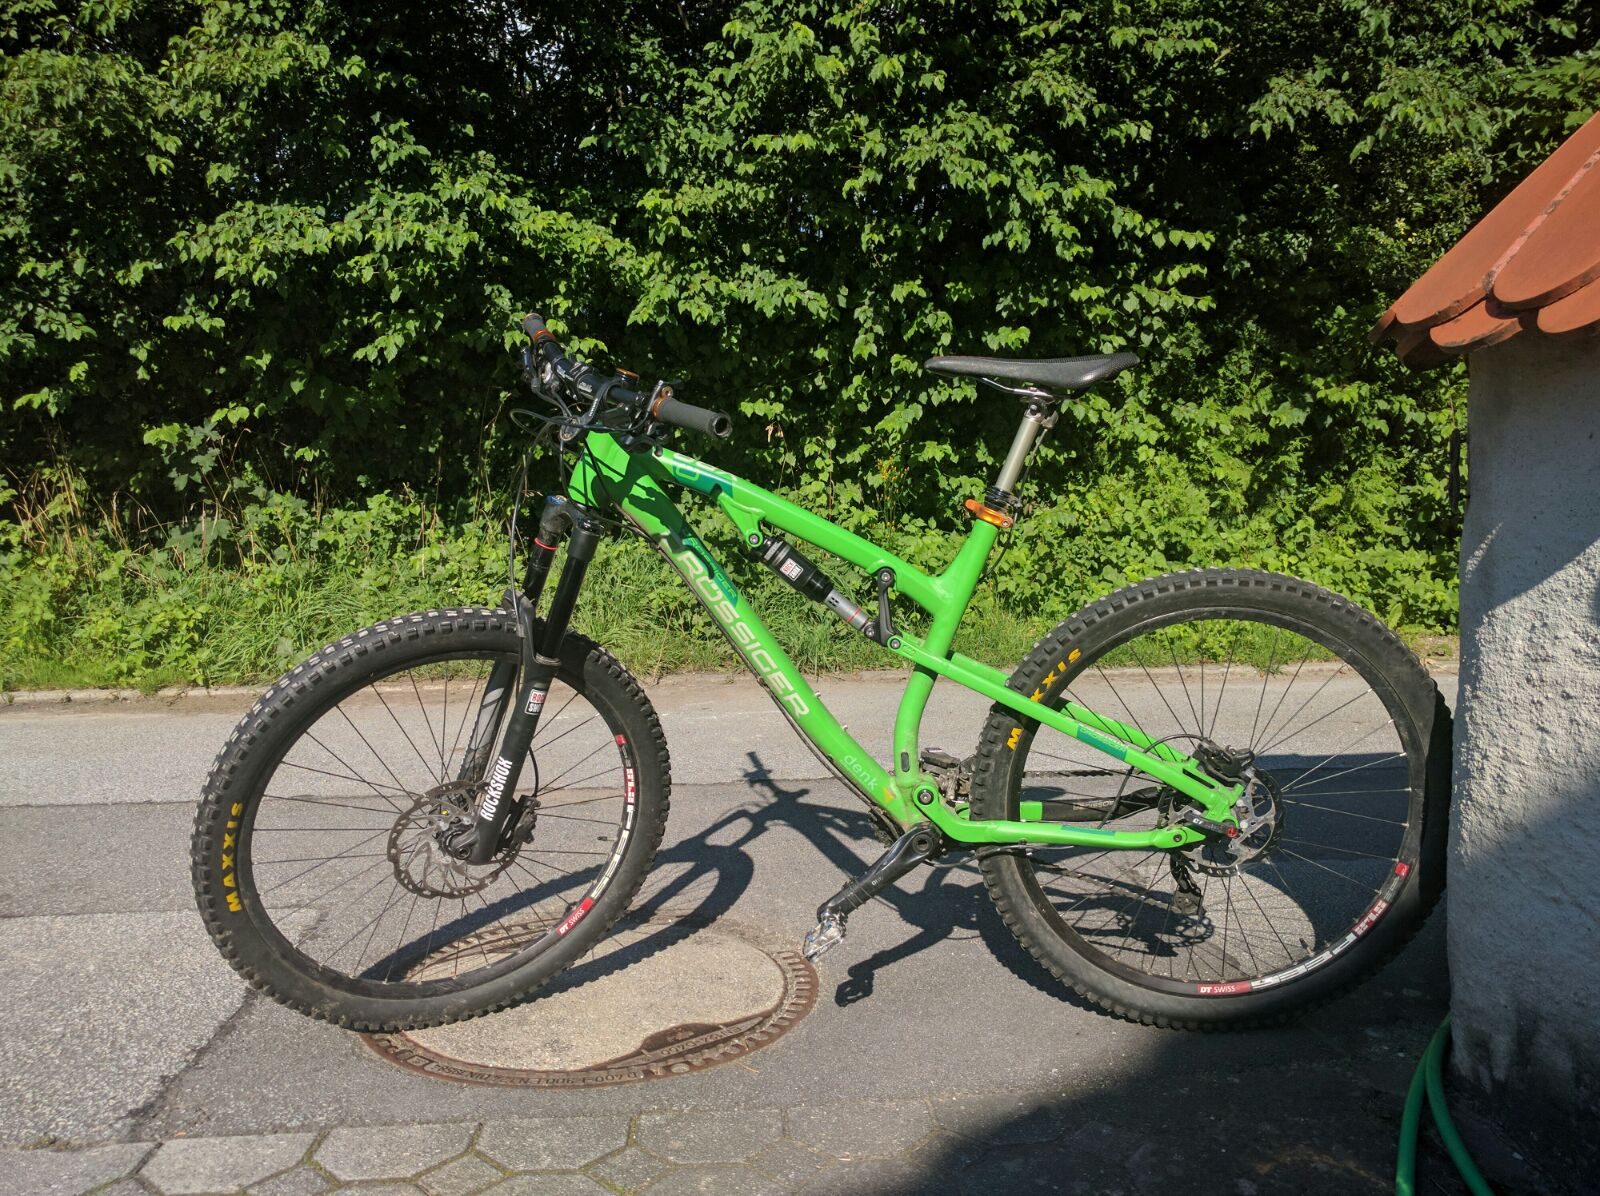
\includegraphics[scale=0.05]{bike_dr}
		  \label{fig:bike_dr}
		\end{center}
		\end{figure}

		\item \textbf{Rotwild G1 2016}: full suspension Downhill-bike (203mm/203mm suspension)

		\begin{figure}[H]
		\begin{center}
 		  \includegraphics[scale=0.05]{bike_rw}
		  \label{fig:bike_rw}
		\end{center}
		\end{figure}

	\end{itemize}
	%bike pictures
	In order to fix the smartphone on the bike, it is recommended to buy a smartphone fix to safely fix your phone on the handlebar. One good possibility is the mumbi TwoSave smartphone fix depicted in \autoref{fig:smartphone_fix}:
	
	\begin{figure}[H]
		\begin{center}
 		  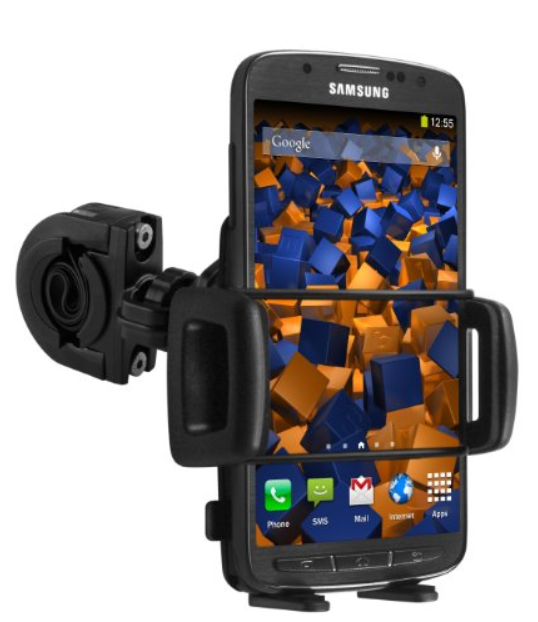
\includegraphics[scale=0.3]{smartphone_fix}
		  \caption{mumbi TwoSave smartphone fix}
		  \label{fig:smartphone_fix}
		\end{center}
	\end{figure}
	\noindent
	It is suitable for many modern smartphones and provides a good multiple-fixing system so your phone will be well protected.\\
	Last requirement is of course that our \textbf{Mission:Chuckhole} app is installed on the used phone.
	During development, we used mostly two different devices: a Samsung Galaxy S4 Active and a Google Nexus 5X.
	On both devices, the app ran smoothly and without any problems.


    \section{Basic Implementation idea}
	
	In order to determine the quality of roads, we will use the g force physical notion. 
	It represents the force that acts somehow on every object that is moving. 
	In context of \textbf{Mission:Chuckhole}, the forces are measured that act on the smartphone.
	From these values, it is possible to detect great changes, which can be interpreted as chuckholes.
	Android phones are equipped with an acceleration sensor that provides values for the forces acting in x, y and z direction.
	Each g force value calculated of these three single values will be associated with a corresponding location provided by GPS.
	The data will be stored locally into an SQLite database to access them again in future app launches.\\
	\autoref{fig:arch_flow} gives an overview of the main parts of \textbf{Mission:Chuckhole}:
	
	\begin{figure}[H]
	\centering
    	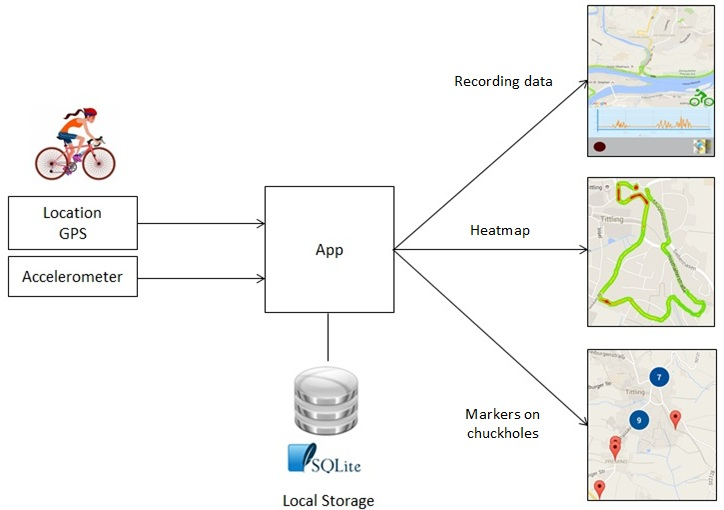
\includegraphics[scale = 0.8]{pic1}
    	\caption{Architecture and flow of information of the app }
	\label{fig:arch_flow}
    	\end{figure}
    
	\noindent
	The next section describes these app features more detailed.
    
    \section{App components and features}
	% pictures etc. here
    
    
    \subsection{Onboarding}
    	Users who launch the app for the first time will start with an initiation to get an overview about the mode of operation and main functionalities of the app. In subsequent uses, this phase will be skipped.\\
    	The first onboarding screen will show the user how to start recording. By pressing the green bike picture, the next onboarding screen will be shown. \\
    	The second screen explains the live visualization graph of g force values that will be displayed during recording.\\
    	Finally, the 'heatmaps and markers overlay' features is introduced.\\
	The onboarding sites are shown in \autoref{fig:onboarding}:
    

	\begin{figure}[H]
	  \centering
	  \subfloat[Onboarding site 1]{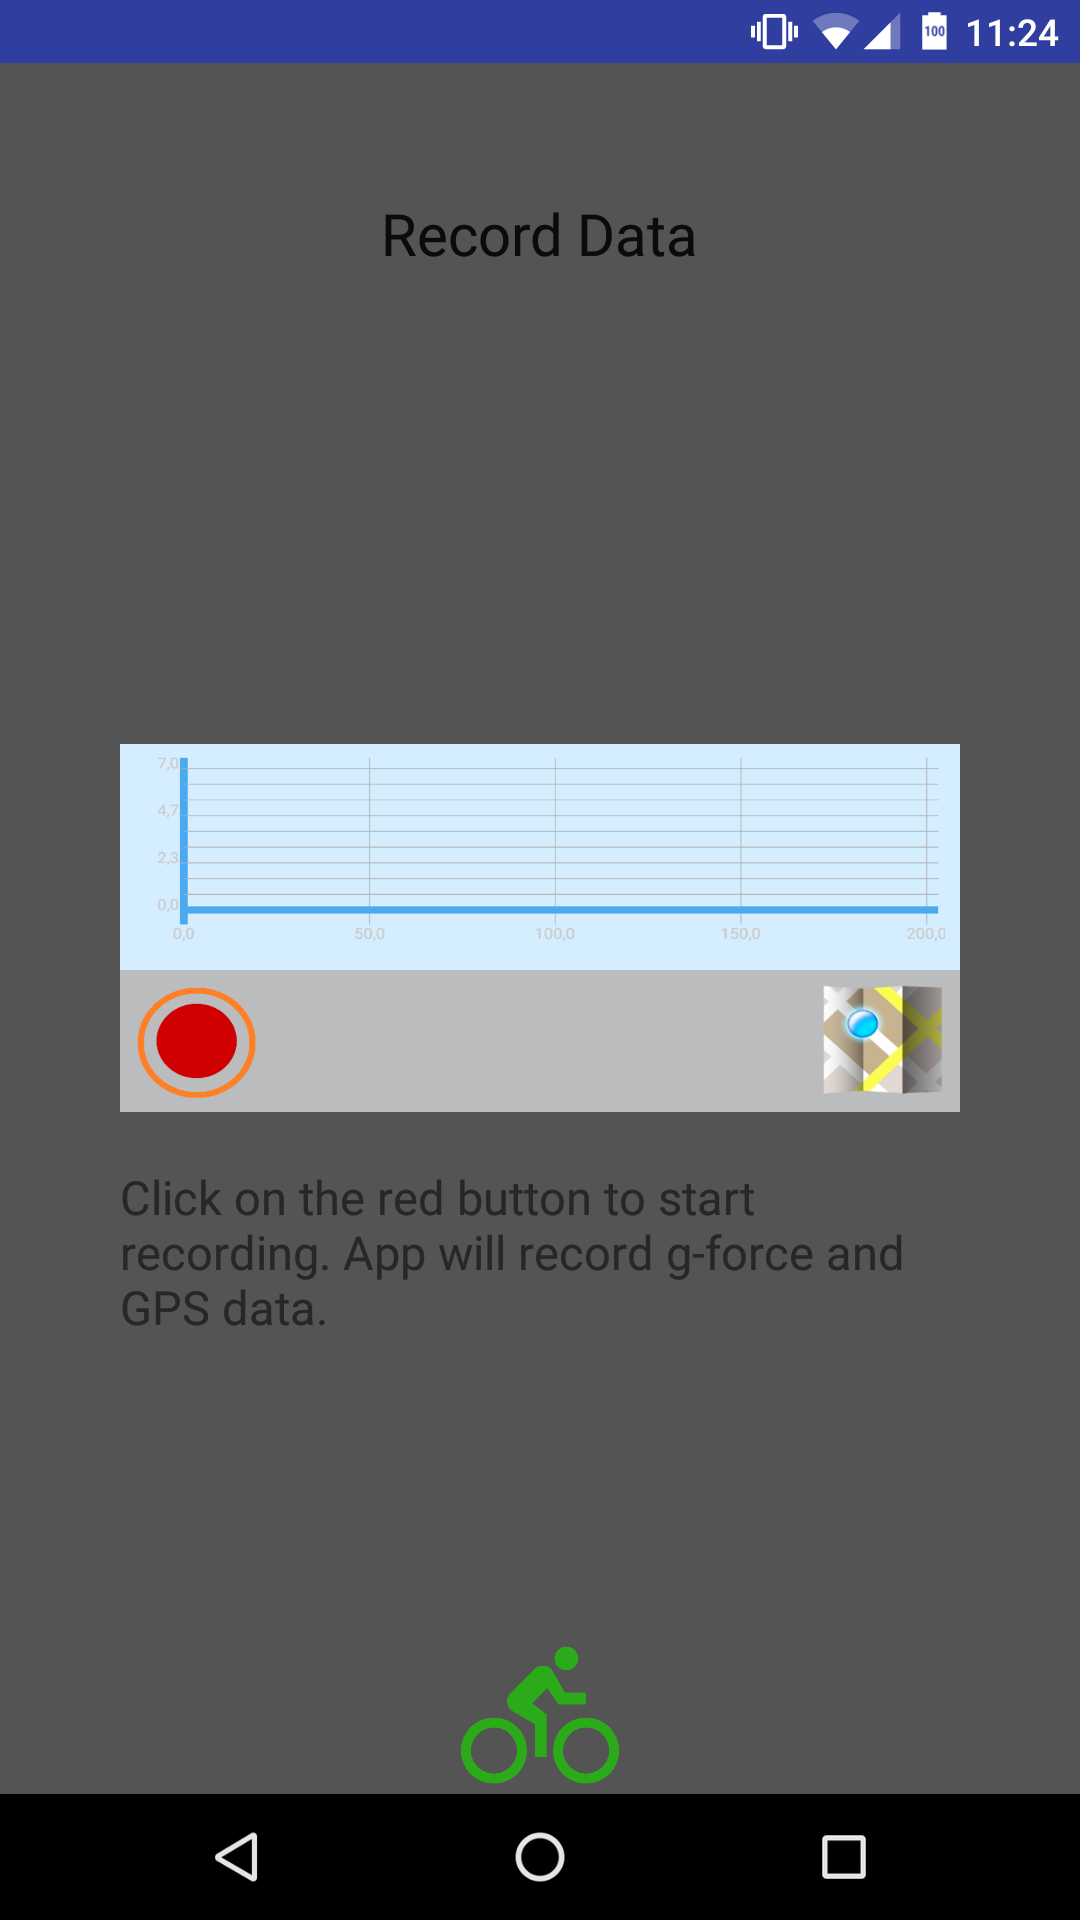
\includegraphics[width=0.25\textwidth]{pic7}\label{fig:onboarding_1}}
	  \hfill
	  \subfloat[Onboarding site 2]{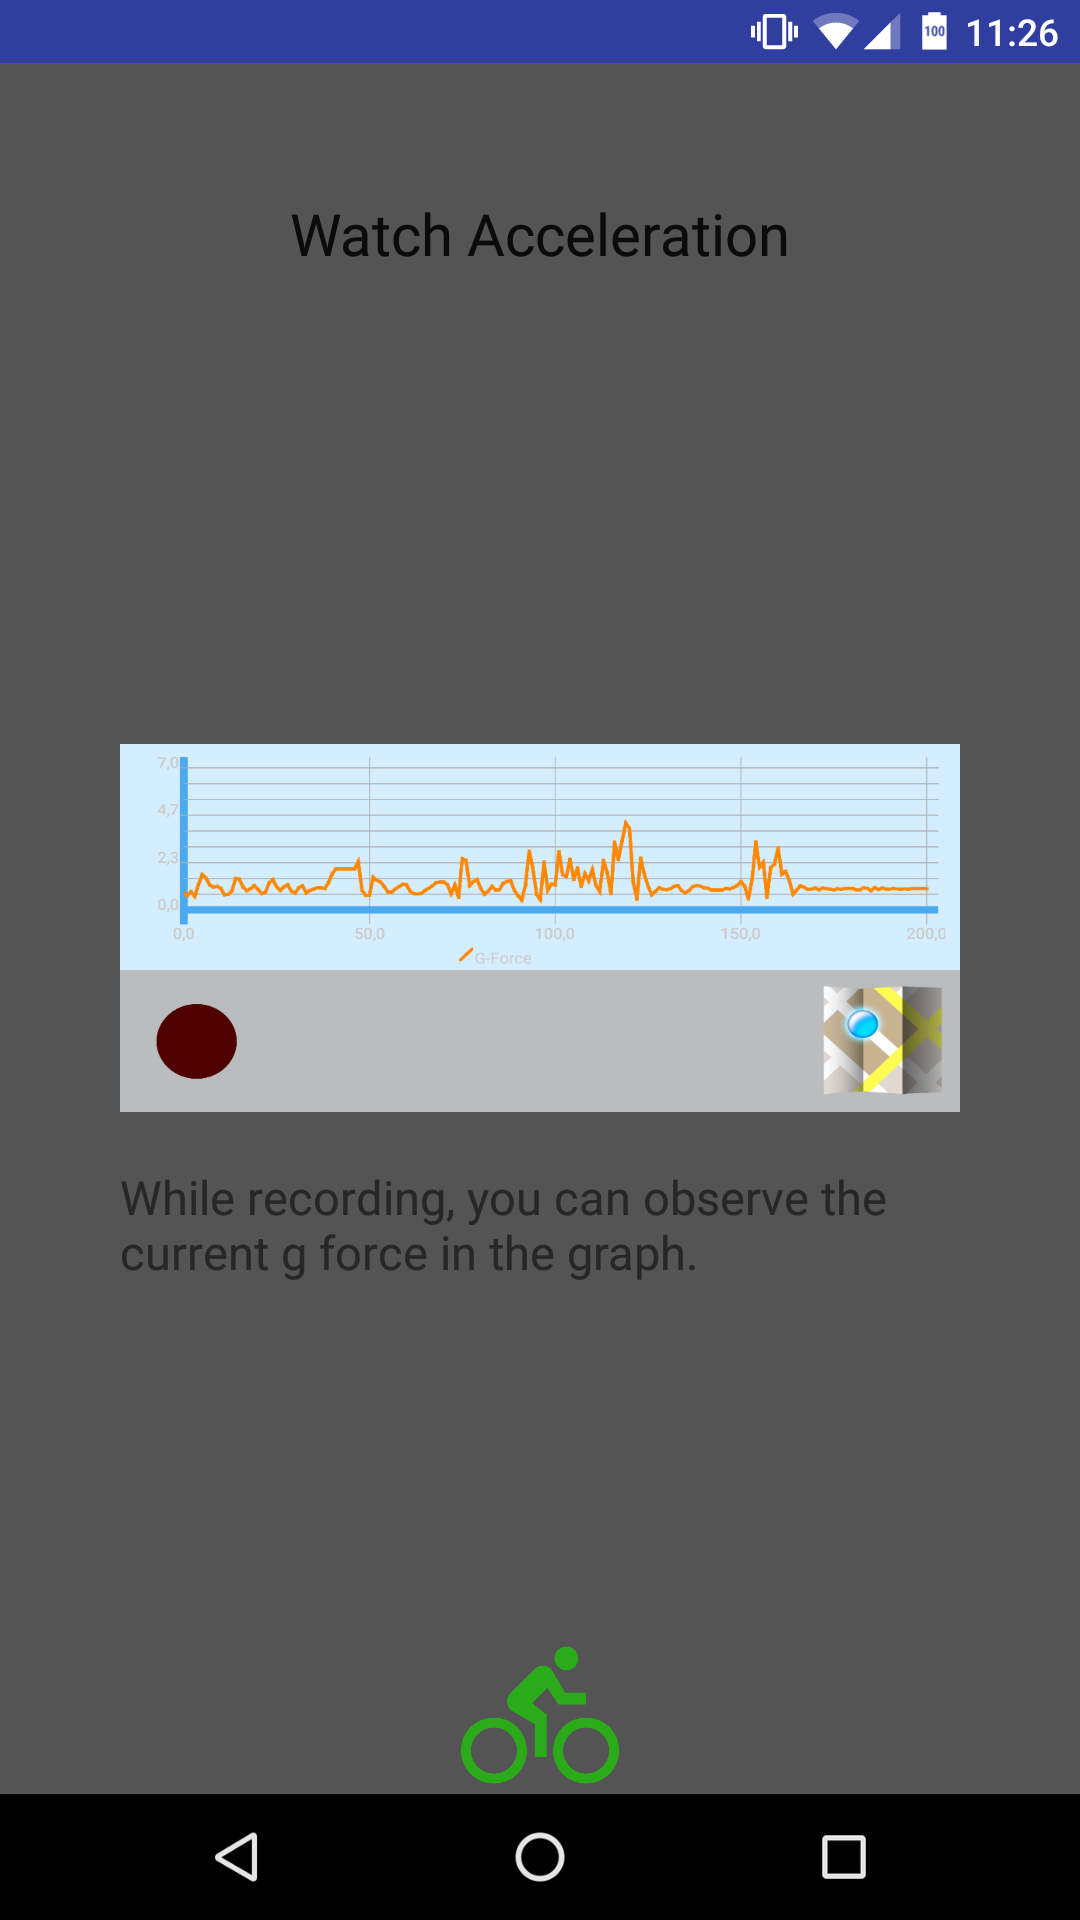
\includegraphics[width=0.25\textwidth]{pic8}\label{fig:onboarding_2}}
	  \hfill
	  \subfloat[Onboarding site 3]{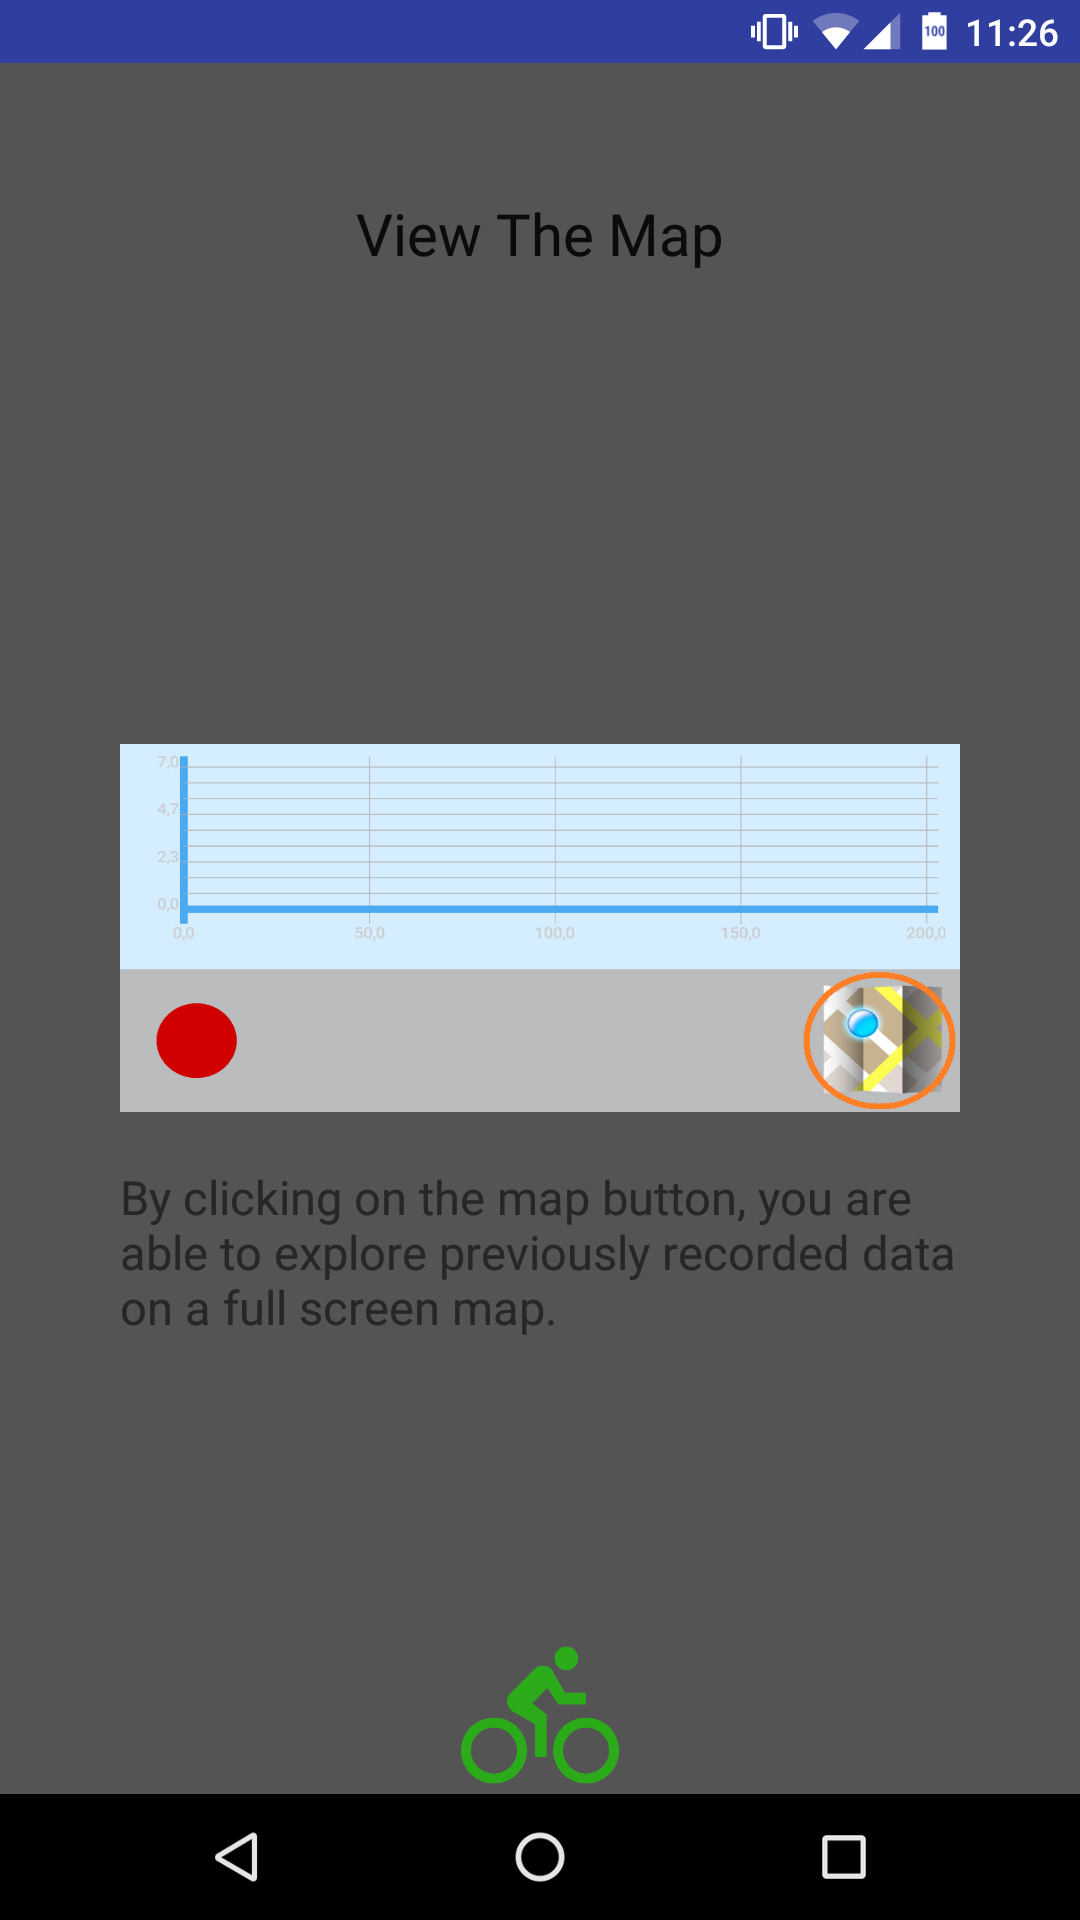
\includegraphics[width=0.25\textwidth]{pic9}\label{fig:onboarding_3}}
	  \caption{Onboarding at first App start}
	  \label{fig:onboarding}
	\end{figure}
	
	
    

    \subsection{Recording data}
    	The recording feature of the app is the important step for gathering data which is then used to display overlays that indicate the quality of roads.
    	Using the accelerometer sensor, the app will get the three acceleration axes' values (x, y and z) that are necessary to calculate the g force by applying the following formula:

    
	\begin{center}
		$ gforce = \frac{\sqrt{x^2 + y^2 + z^2}}{gforce\_earth} $
	\end{center}
	
    	\autoref{fig:record_data} shows the start screen of \textbf{Mission:Chuckhole} in the recording phase:

	\begin{figure}[H]
	  \centering
    	  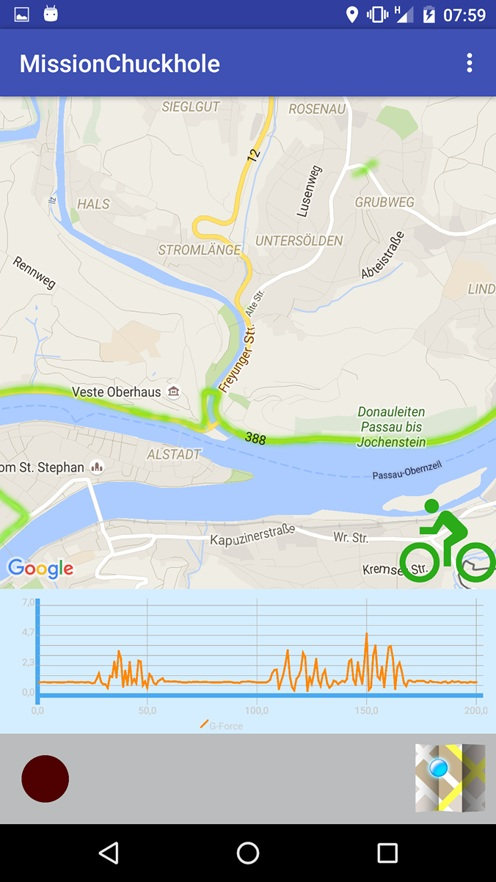
\includegraphics[scale=0.4]{pic2}
    	  \caption{Recording data during a bike ride }
	  \label{fig:record_data}
    \end{figure}
\noindent
    	A tap on the red recording button in the lower left of the start screen starts the recording process.
    	For a better visual distinction, the button changes its color to a darker red.
	At the same time, a green bycicle and its rider show up in the lower right corner of the map.
	Below the map, a grah shows a course of the g force values of the last seven seconds.
	During recording, the heatmap overlay of the map is updated every 10 seconds to observe the most recent results of the recording process.
	A repeated tap onto the recording button stops the recording and opens the big map view.
	
    
    	
    	
    
    
    



    \subsection{Map View}
    	In order to give the user the opportunity to easily view the quality of roads, the recording results get displayed on a map. The application uses the Google Maps Android API that automatically handles access to Google Maps servers, data downloading, map display, and response to map gestures. 
    Additionally, the API is used to add heatmap and markers overlay in clusters.
	% more on this!


    \subsection{Data Storage}
    \textbf{Mission:Chuckhole} uses data from previous runs in order to be able to show as much information as possible to users.
    	Therefore, DataStore is an intermediate data structure between the app features and the SQLite database:\\
	The recorded data is handed over to the DataStore that handles storing to an SQLite database.
	At every new app start, the data from the database is retrieved by the DataStore and can be used again to create overlays.    

    
    \subsection{Heatmap Overlay}
    

	Heatmaps make it easy to understand the distribution and relative intensity of data points on a map.
	In the context of this application, heatmaps are used to represent the quality of roads: green segments indicate rather smooth roads, reddisch segments may be a signal for bumpy roads.
	\textbf{Mission:Chuckhole} uses the Google Maps Android Heatmap Utility to achieve this.\\
    	We opted for a dynamic heatmapping that requires a collection of weighted latitude/longitude coordinates, each with an intensity value that will determine its associated color.
    	The highest values of intensity will be mapped to red while low ones to green. Concerning the values in between, the given color is generated using interpolation between red and green. \\
    	The values that will be displayed are in the format of an AccFix that holds both values from the acceleration sensor (including g force, which represents the intensity) and Location data, provided by the GPS sensor.
	\autoref{fig:heatmap_overlay} shows an example overlay after a bike ride:
     
    \begin{figure}[H]
    \centering
	   
       	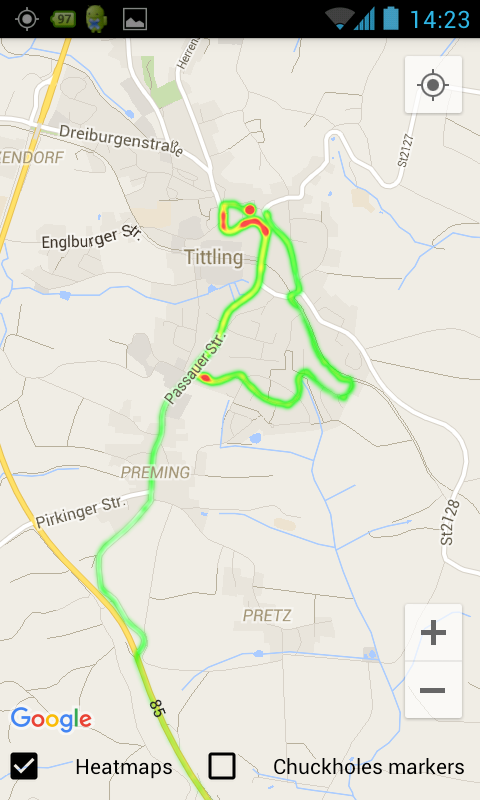
\includegraphics[scale = 0.31]{pic4}
       	\caption{Heatmap overlay example}
	\label{fig:heatmap_overlay}
       
    \end{figure}
    
    
    
    
    
    \subsection{Markers on chuckholes Overlay}
    
    This feature is the second option of an overlay available in the application. The locations are retrieved from the DataStore described previously. Using the Google Maps Android Marker Clustering Utility, a marker will be added for each location where the corresponding g force level reaches or exceeds a specific threshold value. This value has been determined in the pre-evaluation steps and can be changed through the Settings. \\
    When a user views the map at a high zoom level, individual markers will be shown on the map. When a user zooms out, the markers gather together into clusters, to make viewing the map easier. This effect can be recognized in \autoref{fig:markers_overlay}.
    
    \begin{figure}[H]
    \centering
	
	   
       	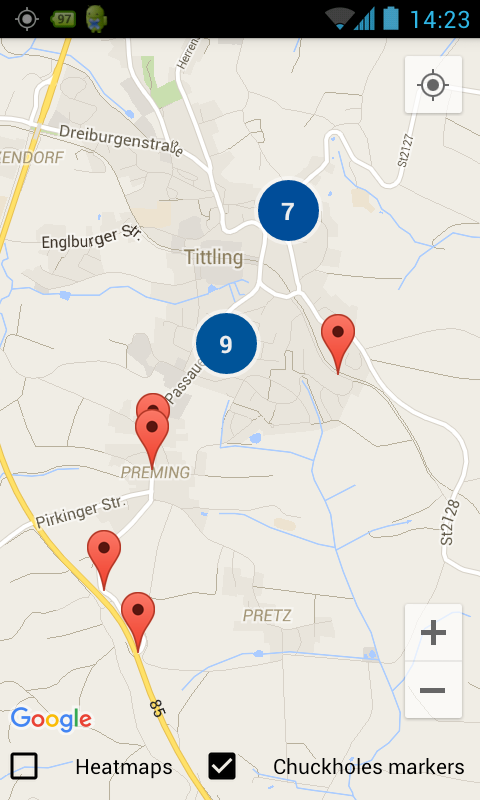
\includegraphics[scale=0.31]{pic3}
   	\caption{Markers on chuckholes in clusters}
	\label{fig:markers_overlay}
	\end{figure}
    
    

    
    

    \section{Problems/Lessons Learned}
	\subsection{Problems}

	%\cite the article
	Unfortunately, the heatmap way of working suffers from some limitations concerning our use case \cite{limitation}. The heatmap's circles overlap at low zoom levels which causes false coloring which occurs due to the fact that the intensity-parameter is additive: the overlap area of two circles of intensity 1 will lead to an overall intensity 2. \autoref{fig:overlaps} illustrates this behavior:
    
    \begin{figure}[H]
    \centering
	   
       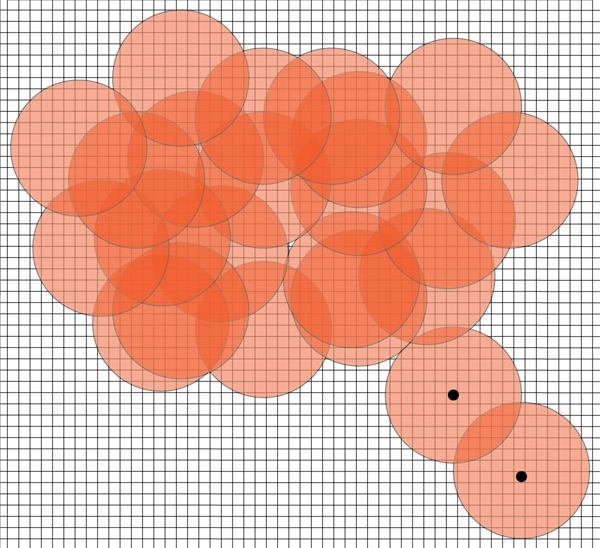
\includegraphics[scale =0.4]{pic6}
    \caption{Overlaps of heatmaps' circles at low zoom levels}
		  \label{fig:overlaps}
       
    \end{figure}
    \noindent
    To overcome this issue, we apply a filtering on our dataset, within a specific zoom range where the overlaps occur, in an attempt to reduce fake coloring of heatmaps.

	\subsection{Lessons learned}

	%more on this: what are the limitations?
	This project was a good occasion to check out the Google maps API for android. However, it suffers from few limitations like unhandled exceptions, leakage of memory, or some rendering problems so it is recommended to review  the releases’ notes and updates before and during any implementation process.

    
    
    
    % bib stuff
    \nocite{*}
    \addtocontents{toc}{\protect\vspace{\beforebibskip}}
    \addcontentsline{toc}{section}{\refname}    
    \bibliographystyle{plain}
    
    \bibliography{Bibliography}

    
    
    
    
\end{document}
